%% Begin copyright
%%
%%  /home/jrf/Documents/books/Books20/Docs/Hjs/library.tex
%%
%%   Part of the Books20 Project
%%
%%   Copyright 2022 James R. Fowler
%%
%%   All rights reserved. No part of this publication may be
%%   reproduced, stored in a retrival system, or transmitted
%%   in any form or by any means, electronic, mechanical,
%%   photocopying, recording, or otherwise, without prior written
%%   permission of the author.
%%
%%
%% End copyright


The Harlan J.~Smith Book Collection at the McDonald Library numbers
over 500 items with 501 catalogued entries. Note however, that a
number of the catalogued entries consist of multiple reprints and
articles or refer to multi-volume works.

The first books were sent to the McDonald library in ????.  I saw a
paper copy of an inventory of the collection a number of years ago but
I have been unable to relocate that list. My cataloguing of this first
set was begun on 1 Dec 2021 and finally finished on 23 Oct 2022 after
a long delay. There were 298 items found in this original collection.

A second set of 4 books were sent by Nat Smith on 2 November 2021.
Cataloguing occured 10--11 April 2022. There were 4 boxes and 57 items
in this second shipment. A third set of books was received from
Jeffrey Mallon on 29 March 2022. These were catalogued on 9--10 April
2022. There were three boxes and 94 items in the third
shipment. Finally, a fourth shipment was received on 13 April 2022 and
catalogued on 16--17 April 2022. There were two boxes (1 cu ft) and
one small box (1/2 cu ft) with a total of 54 items in the fourth
shipment.

\begin{wrapfigure}{r}{0.5\textwidth}
  \centering
  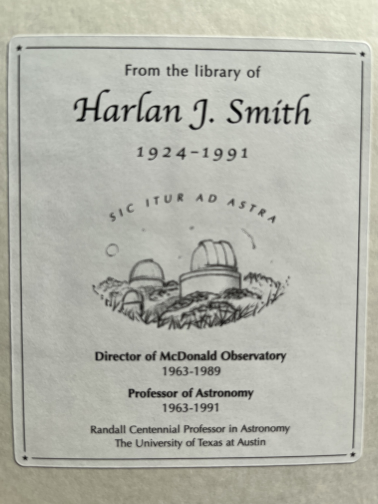
\includegraphics[width=0.48\textwidth]{hjs_bookplate_small.png}
  Bookplate from the HJS library. Designed by Joan Smith.
  \label{fig:bookplate}
\end{wrapfigure}

Many of the items contain a bookplate \textbf{`From the library of
  Harlan J.~Smith'}.  This bookplate was designed by Joan Smith and
added to the books when they were first sent to the McDonald
Library. The bookplate shows Mt.~Locke as viewed from the north-east
with the 107 inch Harlan J.~Smith telescope in the foreground, the 82
inch Otto Struve telescope behind it, and the 36 inch telescope in the
small dome to the left.The Latin inscription \textit{``Sic itur ad
  astra''} translates as \textit{``So we go to the stars''}.

Many of the books also contain the library stamp of Harlan J.~Smith,
usually on the title page. These personalized stamps were quite
popular in the 1970s. This stamp was added by Harlan. In addition,
there is usually a signature or initials of Harlan on the front free
end paper, though occasionally it may appear elsewhere.

A number of books appear to have been purchased from used book dealers.
There are also a number of duplicate books to be found among all the
entries.

Harlan's interests, as indicated by books, are primarily in planetary
studies and space exploration and development. But there are also
works on the history of astronomy, philosophy of science, life on
earth, alien intellegence. and the colonization of space. There is
also a strong interest in climate change dating back to the 1970's.
A number of reports are from his work with the various boards and
committees that he served on.

The catalogue is sorted by year and author. The HJS catalogue number
is ``HJS Shipment\#.Box\#.count'' where shipment 1 is the existing
collection at McDonald while shipments 2, 3, and 4 where the later
boxes shipped in 2021/22. The catalogue entry format is,
\newline

\vbox{%
  \vspace*{0.5 cm}
  \noindent
  {\footnotesize{index}} \textsc{Author(s)} \bookfont{\bfseries Title}

year, place, publisher,\hspace{1em}pagination

edition if known

series name if a part of a published series

publishing comments

comments about the condition of the item

ownership marks of HJS

HJS catalogue number
}


